\documentclass[prb,preprint]{revtex4-1} 
\usepackage{tikz}
\usepackage{amsmath} 
\usepackage{amsfonts} 
\usepackage{graphicx} 
\usepackage{float}
\usepackage{color}
\usepackage{ulem}

\begin{document}

\title{Rotating Polarization of Laser Light Using a Medium in a Magnetic Field}

\author{Ed Lipchus}
\email{ejl13@hampshire.edu} 
\affiliation{Department of Physics, Hampshire College, Amherst, MA, 01002}

\author{Jiajun Shi}
\email{jshi15@amhesrt.edu}
\affiliation{Department of Physics, Amherst College, Amherst MA, 01002}

\date{\today}

\begin{abstract}

As observed by Faraday, when passing light through certain materials, one can change its polarization by applying a magnetic field. Each material has a Verdet Constant, which determines  the degree to which the applied magnetic field will alter the polarization angle. \textcolor{red}{the verdet constant doesn't physically determine the magnitude of the shift in polarization. That depends on the nature of the birefrigent material through which the light is passing. Try ``characterizes'' or ``measures''}In our experiment, we passed a red (650nm) laser beam through a glass rod centered within a solenoid and measured the relative change in angle with respect to a rotating polarizer caused by applying a series of different magnetic fields.\textcolor{red}{was the light from the laser beam polarized or unpolarized? Also, as written, this reads as if the magnetic field caused the 2nd polarizer to rotate} We then solved for the Verdet constant of the glass rod using two different \textcolor{blue}{\textit{mathematical}} methods and compared the results to the accepted values for the glass. \textcolor{red}{this reads as if you used one measurement method and then came up with two different numerical results. That would be disturbing. You actually used two different \textit{experimental} methods (which then also required different method to calculate the Verdet constant)} Our two methods yielded a $v_c$ of -20.53 $\pm$ 0.382 $\frac{rad}{m*T}$ and 18.67 + 0.504 $\frac{rad}{m*T}$, compared with the accepted value of 23 $\frac{rad}{m*T}$. \textcolor{blue}{note: 20.53 - 18.67 = 1.86, while 0.38 + 0.50 = 0.88, so results agree within two standard deviations, if you used standard deviation as your measure of error. I assume you meant a postive value of 20.53 rather than the -20.53 value listed above?}\textcolor{red}{this ``accepted'' value is for a particular material at a particular wavelength, and not actually the same wavelength as you used. I think 670 nm instead of 650? And the Verdet ``constant'' is wavelength dependent. OK to note that this is close to the value reported by Teachspin for a similar rod at a slightly different wavelength, but what you really need to address here is whether or not \textit{your} two measurements are consistent with each other (and those of your classmates) --- or alternatively, within how many standard deviations ---  and if not, whether one of these might be more susceptible to systematic error. }

{\color{blue}Comments on Abstract:
\begin{enumerate}
  \item  You should decide on whether you want to call it the \textcolor{magenta}{Faraday Effect} or the  \textcolor{magenta}{Faraday Rotation} or the \textcolor{magenta}{Faraday equation}, or if you want to use multiple terms, then define faraday rotation in terms of the faraday effect.   
  \item Need sentence describing how you used a second polarizer to determine the angle of polarization (or relative angle of polarization, or shift in polarization) of the light from the change in light intensity after it passed through the material
  \item Need a sentence or two explaining (1) how you detected the relative intensity of the polarized light by measuring the current output from a photodiode (or more specifically, the voltage drop across a 1 Kohm resistor in series with the photodiode) and (2) that the voltage output was proportional to the light intensity (as verified by experiment), and that (3) unwanted voltage offsets and fluctuations in measured light intensity with changes in room lighting were eliminated using by (square-wave) modulation of the laser output and phase-sensistive detection of the transmitted light at the modulation frequency (lock-in amplifier) or some similar language 
  \item Your description of the two experiments sounds as if you found two different results for a single mathematical value.   To improve the clarity of your description, I suggest briefly distinguishing between what you varied, what you measured, and what you calculated. For example, in the first of your two experiments,  you measured the sinusoidal variation of polarized light intensity as a function of polarizer angle for a series of magnetic fields ranging from -x tesla to +y tesla, and from that you determined the magnetic-field-dependent phase shift in polarization (or, if you prefer, the magnetic-field dependent change in polarization angle) upon passage through the glass.  In the second experiment, you measured the variation in light intensity at a fixed polarizer angle as a function of magnetic field, and used that to find the shift in polarization induced by the magnetic field.
  \end{enumerate}
 }


\end{abstract}

\maketitle 

\section{Introduction} 

In 1845, Michael Faraday discovered that light and magnetic field interact in medium, in which the latter rotates the light's plane of polarization by an angle linearly proportional to the field, provided that the magnetic field is parallel to the direction of propagation of light. This magneto-optical phenomenon, now called Faraday effect, provided the very first evidence that light and magnetism are connected. In mathematical expression, \textcolor{magenta}{it writes}
\begin{equation}
\label{faraday}
\phi =VBL  (radian)
\end{equation}
\textcolor{red}{better would be:}
\begin{equation*}
\label{faraday}
\phi =v_cBL 
\end{equation*}
or
\begin{equation*}
\label{faraday}
\Delta\phi =v_cBL 
\end{equation*}
or

where L is the length of the medium light goes through, and B is the magnetic field. V here is a material-dependent number called $Verdet$ constant. 
\textcolor{red}{You haven't defined $\phi$!}

\textcolor{magenta}{do you mean ``Mathematically, we write'' or perhaps ``Mathematically, it is described by the following formula'' (or equivalent)? I don't think the magnetooptical phenomenon is doing the writing.} \textcolor{blue}{Also, I suggest that you use $v_c$ instead of $V$ to avoid confusion with voltage. L isn't in radians, and if you want to indicate that the angle is in radians (which can often be assumed) it is best to do that within the text. }. 

To experimentally verify the Faraday equation in our lab, we need to measure the induced polarization of light within a certain transparent material in a magnetic field, and calculate the Verdet constant from the equation, then compare it with the actual Verdet constant specified for our material. We proceed with a laser beam going through a transparent material in a magnetic field, and passing through a adjustable polarizer. The output laser beam is finally collected by a photodiode that indicates the light intensity by generating a voltage that we can measure with a multimeter, linked with a computer to collect data. With each magnetic field setting, we rotate the polarizer and record voltage reading from the photodiode, given that the light intensity is dependent on the polarizer angle. We expect to see a phase shift in the light intensity across different field settings as the magnetically induced polarization is also dependent on the field. It is worth noting that the Faraday effect shall is a relatively small effect with our lab-strength magnetic field.

We use two approaches to model the Faraday effect. One approach is the direct method, in which we find the phase shift in the light intensity and associate it with the magnetic field. This method gives us the Verdet constant directly from the Faraday equation. Another method, called slope method, utilizes the voltage reading at around 45 degrees from maximum on the polarizer to associate the photodiode voltage with the magnetic field. The first method includes the process of sinusoidal fitting of the data using computer software, while the latter requires mathematical manipulation of the Faraday equation. It is expected that the two methods will yield the same Verdet constant value as they are mathematical equivalent. The descriptions of these two methods can be found in the analysis section.

\section{Experiment}

Before we proceed with the Faraday rotation, we first have to determine the magnetic field used for rotation induction. The lab power supply, Keithley 2230-30-1, generates the currents to create magnetic field within the coil, in our case -3A, -2A, 2A, and 3A for a variety of fields to induce different polarization rotations. We also conduct the experiment with no current inside the coil to better observe the change in polarization with respect to the original polarization of the laser light.

Determining the magnetic field within the coil requires a Gauss meter and some reference, a ruler in our case, to find the distance between the tip of the Gauss meter and the center of the solenoid. We measure the length of the solenoid and make sure the meter tip is centered inside, then pull it out to determine the magnetic field at each point inside the solenoid. In this step, we only supply 1A to the solenoid, as we know from Ampere's law,

\begin{equation}
\label{Ampere}
B=\mu nI
\end{equation}

where $n$ stands for turns per unit length, that magnetic field inside the solenoid is linearly proportional to the current, so if we find the magnetic field at a point to be $B_1$ with 1A current supply, we can say the field would be $2B_1$ for 2A, $3B_1$ for 3A, and so on. The measured magnetic field is

\begin{table}[H]
\centering
\caption{Measuring the Magnetic Field Inside the Solenoid}
\begin{ruledtabular}
\begin{tabular}{c c c c c c}
Distance from Center & Magnetic Field\\
\hline
0                    & 106.5 $\pm$ 0.1G \\ 
5.5cm                & 100 $\pm$ 0.1G   \\ 
6.4cm                & 94.9 $\pm$ 0.1G  \\ 
6.7cm                & 90.0 $\pm$ 0.1G  \\ 
7.1cm                & 80.0 $\pm$ 0.1G  \\ 
7.2cm                & 70.0 $\pm$ 0.5G  \\ 
7.8cm                & 50.0 $\pm$ 0.5G  \\ 
8.1cm                & 40.5 $\pm$ 0.5G  \\ 
8.4cm                & 30.0 $\pm$ 0.5G  \\ 

\end{tabular}
\end{ruledtabular}
\label{AnglevsB}
\end{table}

The next step is to insert the glass rod, which serves as the rotation medium in this experiment, into the solenoid. The length reference is again used to make sure the rod is centered inside the solenoid. The length of the glass rod is $10cm=0.1m$, so each end of the glass rod is $0.05m$ away from the center. According to the above magnetic field table, the field undergoes a minor change from the center to $0.05m$ away, namely from 106.5$\pm$0.1G to 100$\pm$0.1G, suggesting that we can safely take the average value of the fields at these two points, 103G, as the approximation of the magnetic field within the glass rod. The magnetic fields under 2A and 3A shall be 206G and 309G, respectively. Reversing the sign of the current also reverses the sign of the magnetic field.

\begin{figure}[H]
    \centering
    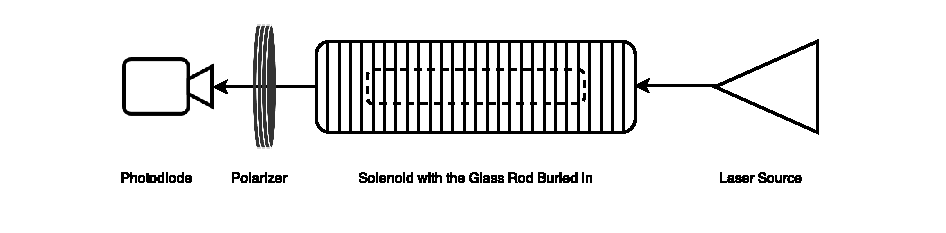
\includegraphics[width=180mm]{ExperimentSetup.pdf}
    \caption{Experiment setup. Drawn not to scale. }
    \end{figure}
    
The initial angle of the polarizer is the angle that allows maximum light intensity. Calling this zero angle, we rotate the polarizer 5 degrees at a time. To filter out any background noise including multimeter noise, background light, and thermal fluctuations within the photodiode, we use several noise reduction devices:

\begin{figure}[H]
    \centering
    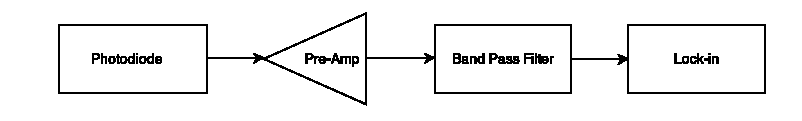
\includegraphics[width=180mm]{Filter.pdf}
    \caption{Noise reduction procedures. The output voltage goes through a pre-amplifier, then a band-pass filter, and finally a lock-in amplifier to eliminate any thermal fluctuations. The room light interference, a systematic error, is minimized by zeroing the multimeter with the room light on.}
    \end{figure}

\section{Analysis and Discussion}
After collecting data for all five different currents, those points were plotted and fit using the plot.ly interface (see Fig.\ref{wave_plot}). Given the positive, periodic nature of the photodiode intensity, we used the following as the fit parameter:
\begin{equation}
\label{volt eqn}
v_d = v_0*cos^2(\theta -\theta _0)
\end{equation}
In this manner, by comparing the phase shift $\theta_0$ for each trial, we can find the relative change in polarization resulting from each magnetic field. For error in relative polarizer angle, we considered $\pm$ 1 degree, however when fitting across all 72 points, their combinations constrained the error by a factor of $\frac{1}{\sqrt{72}}$ for an effective error of $\pm$ 0.118 degrees. Error in voltage, and thus in magnetic field, is considered negligible based on the precision and stability of our power supply and volt meter. In all cases, degrees were converted to radian at a factor of $\frac{\pi}{180}$ for calculating the Verdet constant.

With the photodiode voltage, relative polarizer angle, and magnetic field strength data, there are two possible methods for calculating the Verdet constant:
\begin{equation}
\label{verdet eqn}
v_c=\frac{1}{L}\frac{d\theta }{dB}=\frac{1}{L}\frac{\Delta \theta }{\Delta B}
\end{equation}

\begin{table}[H]
\centering
\caption{Relative Angle vs Magnetic Field}


\renewcommand{\arraystretch}{1.8}
\begin{ruledtabular}
\begin{tabular}{c c c c c c}
Phase Shift (deg) & Fit Error & $\Delta$ Phase Shift (deg) & Current (A) & Magnetic Field (T) & $V_d$ at 45 deg (V)\\
\hline
-1.690 & 0.1267 & -3.692 & -3.000 & -0.0309 & 0.6739 \\
-0.047 & 0.0950 & -2.475 & -2.000 & -0.0206 & 0.7067 \\
2.002  & 0.1219 & 0.000  & 0.000 & 0.000   & 0.7551 \\
4.534  & 0.1657 & 2.532  & 2.000 & 0.0206  & 0.8283 \\
5.471  & 0.1744 & 3.469  & 3.000 & 0.0309  & 0.8550 \\
\end{tabular}
\end{ruledtabular}
\label{AnglevsB}
\end{table}

\begin{figure}[H]
\centering
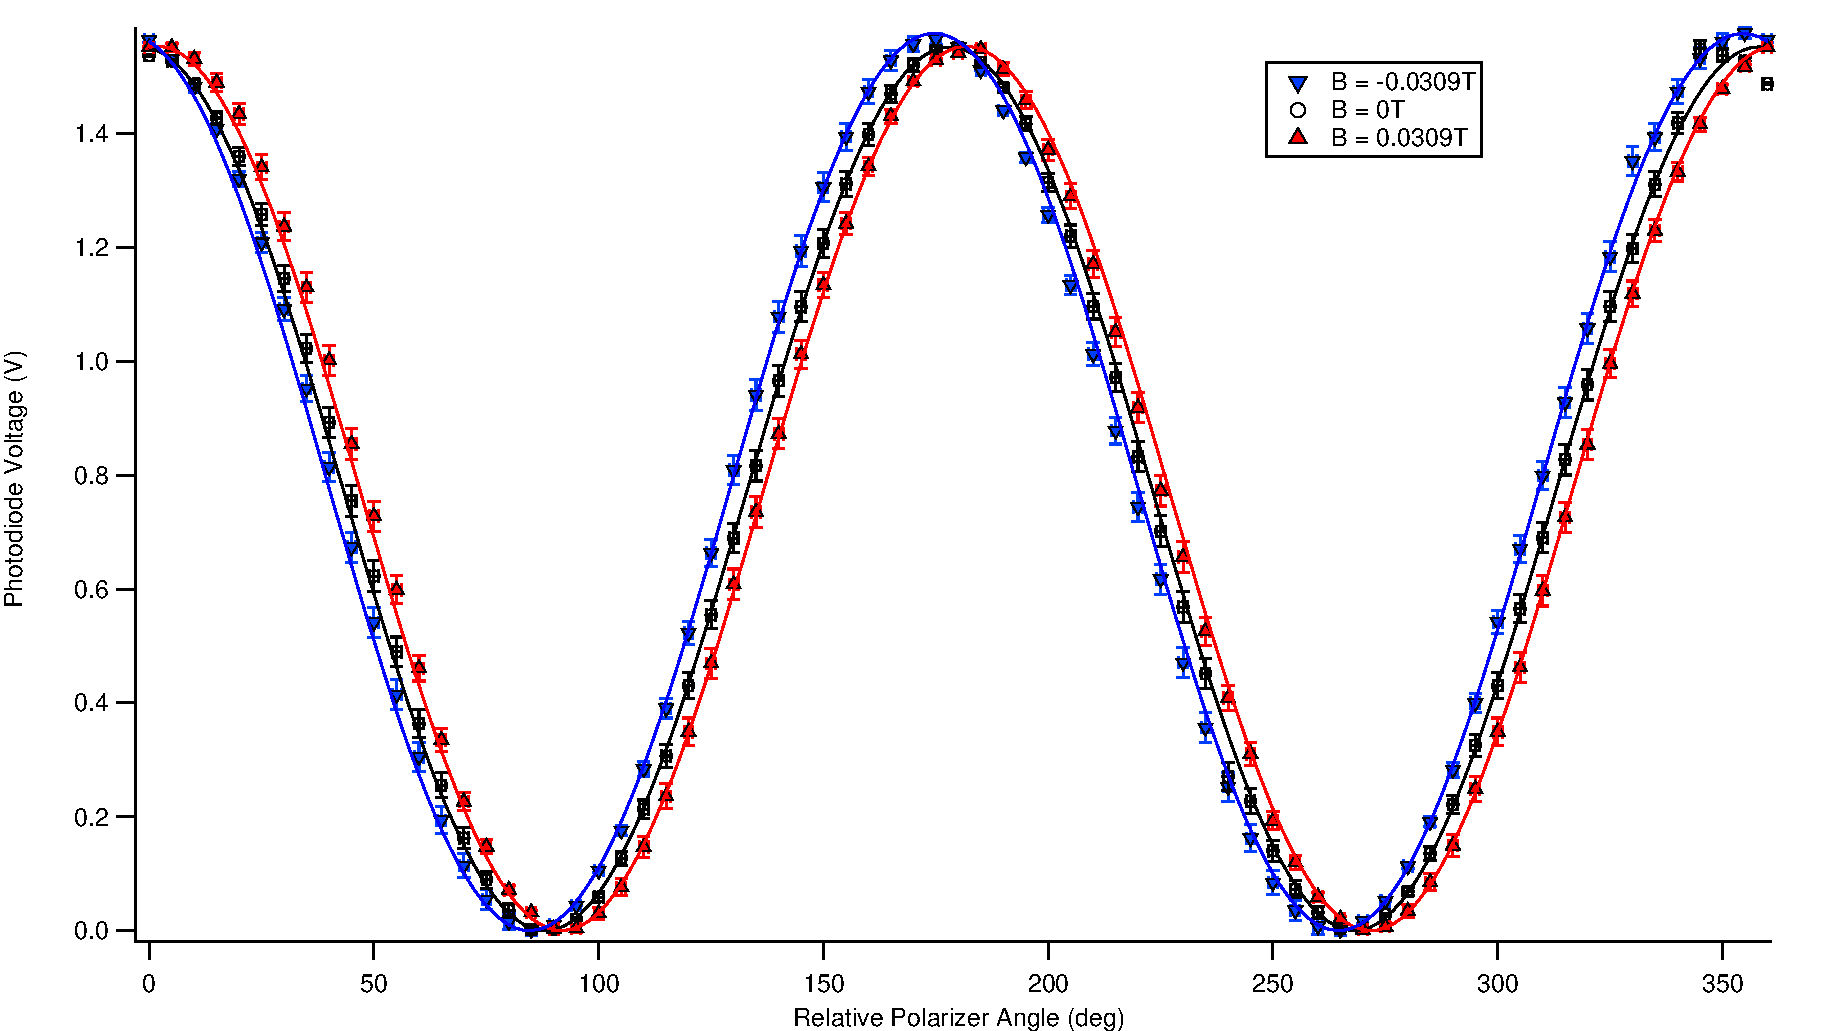
\includegraphics[width=180mm]{FaradaySineWave.pdf}
\caption{Voltage read at the photodiode as a function of relative angle between the polarizer and the laser beam, with best fit lines added. Shown above are the values with no magnetic field applied and with those created by running a current of 3Amps and -3Amps through our solenoid, demonstrating an obvious phase shift between them. Photodiode voltage and phase shifts were also measured under the fields created by running a current of 2Amps and of -2Amps through the solenoid.}
\label{wave_plot}
\end{figure}

The first method attempts to solve for the Verdet constant directly by graphing $\delta \theta$ versus $\delta B$ (see Fig.\ref{V_B Slope}). The slope of the linear fit of this line provides $\frac{\delta \theta}{\delta B}$, solving for $v_c = -20.53$ $\frac{rad}{m*T}$. Error in $\theta$ was calculated as the sum in quadrature of our error in measurement - 0.118 degress - and the error in the linear fit - 2.19 degrees. Neglecting error in B, then $\frac{\delta v_c}{v_c} = \frac{\delta \Delta \theta}{\Delta \theta}$, giving an error of $\pm 0.382$ $\frac{rad}{m*T}$. Thus the direct method yielded a Verdet constant of -20.53 $\pm$ 0.382 $\frac{rad}{m*T}$.

\begin{figure}[h]

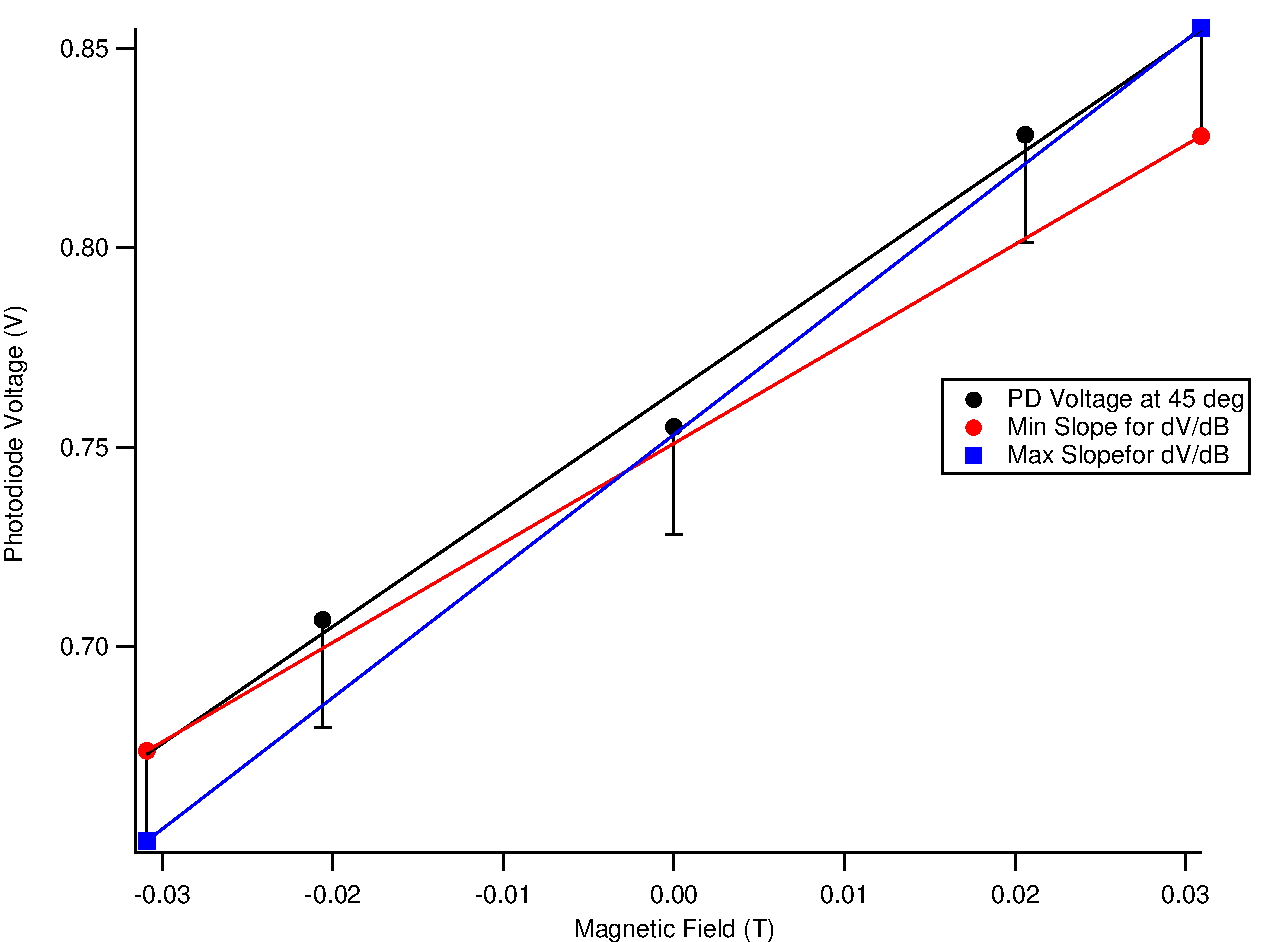
\includegraphics[width=180mm]{V_B_Slope.pdf}
\caption{\label{V_B Slope}Photodiode voltage as a function of magnetic field at a relative polarizer angle of 45 degrees. As an error in either direction of angle would reduce voltage, only down error bars are considered. To get the error in $\Delta$ V/$\Delta$ B, the difference between the best fit slope and the largest and smallest possible fit slopes are calculated.}
\end{figure}

The second method, referred to as the slope method, compares the photodiode voltage to the magnetic field strength instead with the following relation:
\begin{equation}
\frac{dV_d}{dB}= \frac{dV_d}{d\theta }\frac{d\theta }{dB}=v_cL\frac{dV_d}{d\theta }
\end{equation}
From the Verdet equation, we were able to replace the unknown $\frac{d\theta }{dB}$ with the Verdet constant times the length of the glass rod. We can further reduce this equation if we carefully choose a single point at which to analyze this expression. Being a $cos^2(\theta)$ function, the derivative $\frac{\delta V_d}{\delta \theta}$ simplifies very nicely at $\frac{\pi}{4}$ as follows:
\begin{eqnarray}
\label{derivative}
\frac{dV}{d\theta }=-2v_0cos(\theta )sin(\theta )=-v_0sin(2\theta )\\
\frac{dV}{d\theta } \mid_{\frac{\pi }{4}}=-v_0
\end{eqnarray}
Plugging that into the previous equation, we get:
\begin{eqnarray}
\label{slope eqn}
\frac{dV_d}{dB}\mid_\frac{\pi }{4}=v_cL\frac{dV_d}{d\theta }\mid_\frac{\pi }{4}=-v_0v_cL\\
v_c=-\frac{\frac{dV_d}{dB}\mid_\frac{\pi }{4}}{v_0L}
\end{eqnarray}
All that is needed is $\frac{dV_d}{dB}\mid_\frac{\pi }{4}$, which can be found by plotting the photodiode voltage at a relative polarizer angle of 45 degrees against corresponding magnetic field strengths. The error in voltage was calculated by applying our error in angle to the best fit trend lines centered at a relative polarizer angle of 45 degrees. From this, we can find the maximum and minimum possible slopes that would fit the set of points for $\frac{dV_d}{dB}\mid_\frac{\pi }{4}$, and use the differences as error in our slope. Because the slope should be at a maximum value at 45 degrees, then at either point above or below that point, the slope will be lower that at 45 degrees. Since this means that any error will result in a lower than expected value, we will only consider the +error. The final result from this method was $v_c = 18.67 + 0.504$ $\frac{rad}{m*T}$.


\begin{figure}[h]
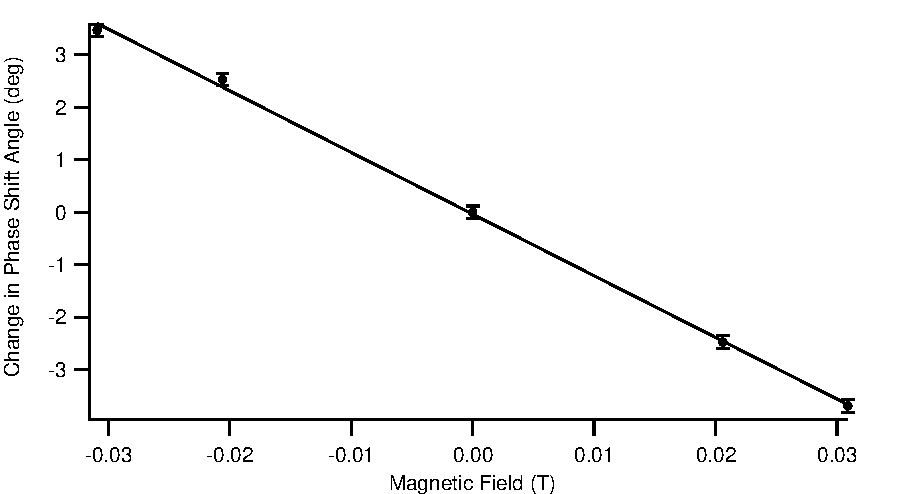
\includegraphics[width=180mm]{dTheta_dT.pdf}
\caption{\label{dTheta_dT}Change in the measured phase shift angle with the application of a magnetic field. The slope of the best fit is used in the direct measurement method of finding the Verdet constant.}

\end{figure}

\section{Conclusion}
The errors in our final values were fairly good: about 2 percent on the direct method and about 3 percent for the slope method. Unfortunately, this means that the two results are inconsistant, as the minimum value for the direct method is 20.15 $\frac{rad}{m*T}$ whereas the maximum value of the slope method is 19.17 $\frac{rad}{m*T}$. While somewhat close, they still are distinctly different. These values are also different from the accepted 23 $\frac{rad}{m*T}$ - being within 10 and 20 percent respectively. When looking at this experiment again, it could be useful to see if there are any changes in Verdet constant for the specific glass used in the rod compared with the general literature for glass, perhaps improving our accuracy. For reducing error even further, a combination of taking more data points and using a device - such as a computer controlled rotater - to be more precise in locking in to the correct angle would help a lot. And while our numbers were lower than expected instead of higher - indicating that zeroing and using the lock-in amplifier were fairly successful in removing contributions from room light - having a way to box in the experiment set-up, thus blocking ambient light, would certainly be beneficial.


\end{document}